%auto-ignore


\chapter{The Ribbon Graph Complex}
\label{cha:ribbon-graph-complex}

In \cite{kontsevich;feynman} and \cite{kontsevich;1993}, M. Kontsevich
introduced ``Graph Homology'' complexes that relate the stable
homology groups of certain infinite-dimensional Lie algebras to
various other topological objects, depending on the choice of an
operad.  In particular, the ``associative operad'' variant of the
construction gives birth to a chain complex whose homology is
isomorphic to the (co)homology of the moduli space of smooth punctured
curves $\M_{g,n}$.

Here we give a construction of the ribbon graph complex, deriving it
as a relative of Harer's arc-system complex
\cite{harer;cohomological-dimension,
  harer;cohomology-of-moduli}\FIXME{Non sono affatto sicuro che gli
  arc-system siano stati introdotti da Harer.  Per\`o non \`e molto
  importante chi li ha introdotti, quanto che qui si costruisce il
  complesso dei grafi a nastro parallelamente a come Harer costruisce
  quello degli arc-system.}, and prove the isomorphism of its homology
with the rational (co)homology of $\M_{g,n}$.  The main ingredient of
this construction is a cell decomposition of $\M_{g,n}$ based on a
theorem of Jenkins and Strebel
\cite{strebel;quadratic-differentials;1983}.  This ribbon graph
complex is the same complex that one gets by applying Kontsevich'
construction in the associative case; however, the proof given here is
specific to $\M_{g,n}$ and does not trivially extend to other cases.

A different construction of the graph complex, complete with full
details, is given in \cite{conant-vogtmann;2003}, closely following
Kontsevich' original work.  In contrast to the simpler method
presented here, the techniques devised by Kontsevich are suitable to
further generalization to any ``modular operad''
\cite{getzler-kapranov}.



\section{Moduli Spaces of Curves}
\label{sec:moduli-spaces}

Let us recap the main points of the construction of the moduli space
of smooth algebraic curves; the short summary given here tracks
closely the first section of \cite{looijenga;cellular-decomposition},
which has proofs and references.

Fix integers $g,n\geq0$ such that $2 -2g - n < 0$. Let $S$ be a Riemann
surface of genus $g$ and $P = \{ x_1, \ldots, x_n \}$ a set of $n$ points
in $S$.  

Let $\Diff(S,P)$ be the group of diffeomorphims of $S$ that fix $P$
pointwise\FIXME{Nella costruzione di $\T{g,n}$ ed $\M{g,n}$ \`e
  richiesto che $\Diff$ fissi $P$ \emph{pointwise}, non
  \emph{setwise}, altrimenti ci ritroviamo con un'azione di $\Perm{n}$
  sulle marcature, che non vogliamo.  Giusto?  Questo \`e cruciale per
  la questione degli automorfismi dei grafi.}; let $\Diff^0(S,P)$,
$\Diff^+(S,P)$ be the subgroups of diffeomorphisms homotopic to the
identity mapping $\id_S$, resp.\ the subgroup of
orientation-preserving diffeomorphisms.

Every set $P$ of marked points can be carried into another chosen one
$P'$ by a diffeomorphism $\phi$ homotopic to the identity mapping
$\id_S$.  Therefore, $\Diff^+(S,P)$ and $\Diff^0(S, P)$ depend only on
$n = \card{P}$ and not on $P$, cf. \cite{krushkal;riemann-surfaces}.
Summing up:
\begin{definition}\label{dfn:diff}
  $\Diff(S,n)$ is the group of orientation-preserving diffeomorphisms
  that keep the $n$ marked points fixed.

  $\Diff^0(S,n)$ is the group of diffeomorphisms of $S$ homotopic to
  the identity mapping $\id_S$ that keep the $n$ marked points fixed.
\end{definition}

Every complex structure  on $S$ determines a conformal structure; let
$\Conf(S)$ be the set of all conformal structures on $S$. 
\begin{definition}\label{dfn:teichmuller}
  The \emph{Teichm{\"u}ller space}
  \begin{equation*}
    \T_{g,n} := \Conf(S) / \Diff^0(S, n)
  \end{equation*}
  is, by definition, the quotient of the set of all conformal metrics on
  $S$ by the set of all diffeomorphisms homotopic to the identity and
  fixing the $n$ marked points.
\end{definition}
The Teichm{\"u}ller space $\T_{g,n}$ is an analytic space and is
homeomorphic to a convex domain in $\setC^{3g - 3 + n}$.

\begin{definition}\label{dfn:mapping-class-group}
  The \emph{mapping class group} $\Gamma_{g,n}$ is the set of connected
  components of $\Diff^+(S, n)$, the group of all diffeomorphisms that
  preserve orientation and fix marked points:
  \begin{equation*}
    \Gamma_{g,n} := \Diff^+ (S, n) / \Diff^0(S, n).
  \end{equation*}
\end{definition}


\subsection{Moduli space of smooth curves}
\label{sec:Mgn}

\begin{definition}
  The topological space $\M_{g,n} := \T_{g,n} / \Gamma_{g,n}$ is named the
  moduli space of (smooth) $n$-pointed algebraic curves of genus $g$.
  It parameterizes complex structures on $S$, up to
  orientation-preserving diffeomorphisms fixing the $n$ marked points.
\end{definition}
Since $\T_{g,n}$ is an analytic variety and $\Gamma_{g,n}$ acts
discontinuously with finite stabilizers, $\M_{g,n}$ inherits a
structure of analytic orbifold of complex dimension $3g - 3 + n$.

\subsubsection{Alternate descriptions of $M_{g,n}$}
\label{sec:alternate-Mgn}
One may instead consider equivalence classes of $n$-punctured surfaces
$S$ (i.e., with $n$ points \emph{removed}) by bianalytic mappings, and
repeat the same construction of the Teichm\"uller and the moduli space.
By the Riemann extension theorem, the two approaches turn out to be
the same.

Conversely, one may want to keep the complex structure on the surface
fixed, while actually moving the punctures; still, this \emph{is} a
way of varying the complex structure on $(C; x_1, \dots, x_n)$. This
approach leads to the construction of $\M_{g,n}$ by equivalence
classes of triples $(C, x, f)$ where $C$ is a complex curve, $x: \{1,
\ldots, n\} \longrightarrow C$ a marking of points, and $f: C \to S$ a homeomorphism with a
fixed reference topological Riemann surface $S$.


\subsection{Moduli Space of Stable Curves}
\label{sec:moduli-space-stable}

Deligne and Mumford \cite{deligne-mumford} showed that $\M_{g,n}$ has
a projective compactification $\Mbar_{g,n}$; this space can be
described as the moduli space of stable curves of arithmetic genus
$g$.
\begin{definition}
  A stable complex curve $C$ is a complete connected curve such that:
  \begin{enumerate}
  \item $C$ has only nodal singularities;
  \item the marked points $x_1, \ldots, x_n$ are nonsingular points in
    $C$;
  \item the pair $(C; x_1, \ldots, x_n)$ has a \emph{finite} automorphism
    group.
  \end{enumerate}
\end{definition}
Equivalently, this last condition can be expressed by saying that:
\textsl{a)} any rational component of the normalized curve $\tilde C$
must contain at least 3 special points (that is, marked points or
singular points); \textsl{b)} any component of genus $1$ must contain
at least 1 special point.

Let $C$ be a stable curve, with $q$ irreducible components and $r$
nodal points. Let $\{C_j\}_{j=1, \dots, \nu}$ be the irreducible
components of $C$ and $g(C_j)$ the geometric genus of $C_j$.  The
arithmetic genus of $C$ is defined by the equation:
\begin{equation*}
  p(C) := \bigl({\textstyle \sum_{j=1}^\nu} g(C_j) \bigr) + r - q + 1.
\end{equation*}

Informally, stable curves are constructed by attaching smooth curves
``by the nodes'', such that the arithmetic genus be $g$ and the total
number of punctures be $n$.



\section{Ribbon graphs}
\label{sec:ribbon-graphs}

Ribbon graphs take their name from being usually depicted as graphs
with thin bands as edges, instead of 1-dimensional lines.  For much
the same reason, they have also been called ``fatgraphs''.

\begin{definition}
  \label{dfn:ribbon-graphs}
  A ribbon graph is a finite CW-complex of pure dimension 1, together
  with an assignment, for each vertex $\gamma$, of a cyclic ordering of the
  edges incident at $\gamma$.  Unless otherwise specified, we assume that
  all vertices of a ribbon graph have valence at least 3.

  A morphism of ribbon graphs $G$, $G'$ is a cellular map $f:G\to G'$
  such that, for each vertex $\gamma$ of $G'$, the preimage $f^{-1}(U)$ of
  a small neighbourhood of $\gamma$ is a small neighbourhood of a tree in
  $G$ (i.e., it is a grpah with no nontrivial homological cycles).
\end{definition}

If $G$ is a ribbon graph, denote $\Vertices{G}$, $\Edges{G}$ and
$\Legs{G}$ the sets of vertices, (unoriented) edges and oriented edges
(at times called ``legs'' or ``half-edges'').

\subsubsection{Morphisms arising from contraction of an edge}
\label{sec:contractions}
Let $G$ be a ribbon graph, and $G'$ be the CW-complex obtained by
contracting an edge $\alpha \in \Edges{G}$ to a point.  $G'$ inherits a
ribbon graph structure from $G$: if $(\alpha < \alpha_1 < \ldots < \alpha_k < \alpha)$ and $(\alpha
< \alpha'_1 < ... < \alpha'_h < \alpha)$ are the cyclic orders at endpoints of $\alpha$,
then the vertex formed by collapsing $\alpha$ is endowed with the cyclic
order $(\alpha_1 < \ldots < \alpha_k < \alpha'_1 < \ldots < \alpha'_h)$.  The contraction morphisms
play a major role in manipulation of ribbon graphs.

\begin{definition}\label{dfn:admissible-contraction}
  If $\alpha$ connects \emph{two distinct} vertices, i.e., it is \emph{not
    a loop}, then we say the contraction is \emph{admissible}.
\end{definition}

\begin{lemma}\label{lemma:contraction1}
  Any morphism of ribbon graphs is a composition of isomorphisms and
  \emph{admissible} contractions of edges. 
\end{lemma}


\subsection{A combinatorial description of ribbon graphs}
\label{sec:rg-comb}

There is an equivalent characterization of a ribbon graph, capturing
the combinatorial and computable aspect.  It will be used
interchangeably with the topological one in the sequel.

\begin{lemma}
  A ribbon graph is uniquely determined by the following data: a
  finite set $L$ together with bijective maps $\sigma_0, \sigma_1, \sigma_2: L \to L$ such
  that:
  \begin{itemize}
  \item $\sigma_1$ is involutive: $\sigma_1^2 = \id$, and
  \item $\sigma_0 \circ \sigma_2 = \sigma_1$.
  \end{itemize}
\end{lemma}
\begin{proof}
  To pass from the topological description to the combinatorial one,
  take $L$ to be the set of \emph{oriented} edges of the CW-complex
  underlying a ribbon graph.  Define $\sigma_1:L\to L$ as the orientation
  reversal on edges.  Define $\sigma_0:L\to L$ by means of the cyclic order
  at vertices: let $L(v)$ be the subset of edges in $L$ that
  \emph{end} at a vertex $\gamma$, the cyclic order on edges incident at
  $\gamma$ induces a cyclic order on $L(v)$.  If $l\in L(v)$ then define
  $\sigma_0(l)$ as the successor to $l$ in the cyclic order on $L(v)$.
  Finally, define $\sigma_2: L \to L$ by means of $\sigma_2=\sigma_0^{-1}\sigma_1$.

  Vice versa, let $L_i$ be the set of orbits of the map $\sigma_i$.  Take
  $L_0$ to be the set of 0-cells; for each $\{l,l'\} \in L_1$, glue a
  1-cell to the 0-cells corresponding to the $\sigma_0$-orbits of $l$ and
  $l'$.  The cyclic order at each vertex is induced by the action of
  $\sigma_0$.
\end{proof}
Any two of the maps $\sigma_0, \sigma_1, \sigma_2$ determine the third, by means of
the defining relation $\sigma_0 \circ \sigma_2 = \sigma_1$; therefore, to give a ribbon
graph, it is sufficient to specify only two out of three maps.

In the combinatorial description, $\Vertices{G}$ is the set $L_0$ of
orbits of $\sigma_0$, $\Edges{G}$ is the set $L_1$ of orbits of $\sigma_1$, and
$\Legs{G}$ is plainly the set $L$.  Denote $\Holes{G}$ the set $L_2$
of orbits of $\sigma_2$; its geometrical significance will be cleared in
the next section.


\subsection{From ribbon graphs to Riemann surfaces}
\label{sec:rg-to-surfaces}

Let $G = (L; \sigma_0, \sigma_1, \sigma_2)$ be a ribbon graph.  When passing to the
topological description, we associate a 0-cell with every $\sigma_0$-orbit
in $L$, and a 1-cell with every $\sigma_1$-orbit.  Extend this procedure
and glue a punctured 2-cell along any $\sigma_2$-orbit: if $\{l, \sigma_2(l), \ldots,
\sigma_2^k(l)\}$ is a $\sigma_2$-orbit (in the order it is swept by $\sigma_2$) and
$\sigma_2^{k+1}(l) = l$, then attach a punctured 2-disk so that its oriented
border is the 1-cycle formed by the graph edges corresponding to
$\sigma_2^i(l)$.

Thus we have constructed a punctured Riemann surface $S(G)$, such that
$G$ is a deformation retract of $S(G)$.  Denote $\Holes{G}$ the set
$L_2$ of orbits of $\sigma_2$; in the topological descpription, its
elements are the support of 1-cycles in $H^1(G)$ that correspond under
the retraction to small loops around the punctures in $S(G)$; they are
called ``boundary components'' of $G$, by abuse of language.  Also in
the topological description, it will be convenient to identify a
boundary component $\beta$ with the set of edges it is made of, and a
vertex $\gamma$ with the set of edges incident to it.

\begin{definition}
  A ribbon graph $G$ is \emph{numbered} when it is endowed with a
  bijection $\{1,\ldots, n\} \to \Holes{G}$.

  It is understood that morphisms of numbered ribbon graphs respect th
  numbering of boundary components.
\end{definition}


\subsection{The genus of a ribbon graph}
\label{sec:rg-genus}

The correspondence between ribbon graphs and Riemann surfaces allows
us to give the following.
\begin{definition}\label{dfn:rg-genus}
  The \emph{puncture number} of a graph $G$ is given by $n =
  \card{\Holes{G}}$, and is equal to the puncture number of the
  Riemann surface $S(G)$.

  If $S(G)$ has genus $g$ and $n$ punctures, then:
  \begin{equation*}
    \chi(G) = \chi(S(G)) = 2 - 2g - n = 2 - 2g - \card{\Holes{G}},
  \end{equation*}
  so we can define, for any ribbon graph $G$, the \emph{genus} $g$, as
  given by the above relation.
\end{definition}

\begin{lemma}\label{lemma:contraction2}
  If $G'$ is obtained from $G$ by an admissible contraction, then $G$
  and $G'$ share the same genus and puncture number.
\end{lemma}

Denote $\RG$ the category of ribbon graphs and their morphisms.  By
lemmas~\ref{lemma:contraction1} and~\ref{lemma:contraction2}, $\RG$
decomposes into the disjoint union of categories $\RG{g,n}$ whose
objects are ribbon graphs of genus $g$ with $n$ punctures:
\begin{equation*}
  \RG = \coprod_{g,n} \RG{g,n}
\end{equation*}
No morphism connects an object of $\RG{g,n}$ with an object of
$\RG{g',n'}$.


\subsection{Embedded ribbon graphs}
\label{sec:embedded-rg}

Fix a reference Riemann surface $S$.

An embedding of a ribbon graph $G$ is a injective continuous map $\iota:G\to
S$, that is, a homeomorphism of $G$ onto $\iota(G) \subseteq S$.

When confusion is likely to arise, we shall speak of \emph{abstract}
ribbon graphs, to mean the topological and combinatorial objects
defined in \csref{dfn:ribbon-graphs}, as opposed to \emph{embedded}
ribbon graphs as in \csref{dfn:embedded-rg} below.

\begin{definition}\label{dfn:embedded-rg}
  An embedded ribbon graph is an equivalence class $[G, \iota,
  \{\psi_i\}_{i=1}^n]$, modulo the action of $\Diff_0(S)$, of triples
  composed of a ribbon graph $G$, an embedding $\iota:G\to S$, and
  homeomorphisms $\psi_i$ of each connected component $C_i$ of $S \setminus \iota(G)$
  with a punctured disk $D_i^\times$ such that $\psi_i\mid_{\partial C_i} = \iota^{-1}$.

  A morphism $[f]$ from $[G, \iota, \psi_*]$ to $[G', \iota', \psi'_*]$ is given by
  the following data:\FIXME{Alla lettera, questa definizione \`e
    sbagliata: non importa quale sia l'omotopia tra $\iota$ e $\iota' \circ f$,
    basta che ce ne sia una.  Ovvero, il morfismo esiste se ce n'\`e
    almeno una, e tutte quelle che esistono sono equivalenti.}
  \begin{itemize}
  \item an abstract ribbon graph morphism $f:G\to G'$;
  \item a homotopy $\eta:[0,1] \times S\to S$, such that $\eta(0,-) = \id_S$,
    transforming $\iota$ into $\iota' \circ f$ and $\psi_i$ into $\psi'_i$.\FIXME{%
      \`E meglio scrivere le condizioni esplicite $\eta(1, \iota(x)) = \iota' \circ f(x)$
      e $\psi_i \circ \eta(1,y) = \psi'_i(y)$\ ?
      }%
  \end{itemize}

  Embedded ribbon graphs with their morphisms form a category $\ERG$.
\end{definition}
In other words, an embedded ribbon graph is a ribbon graph $G$ endowed
with a homeomorphism ${\tilde \iota}$ between $S(G)$ and the ambient
surface $S$ (modulo the action of $\Diff^0(S)$).\FIXME{%
  Meglio usare questa come definizione, e usare \ref{dfn:embedded-rg}
  come caratterizzazione?  Questa richiede di fissare $S$ come
  superficie topologica una volta per tutte, quindi conduce a una
  costruzione dello spazio dei moduli come triple $(C,f,S)$ similmente
  a quanto fa Harer?}%
Since a morphism $f:G\to G'$ of abstract ribbon graphs extends trivially
to a morphism ${\tilde f}:S(G)\to S(G')$, then a morphism of embedded
ribbon graphs is determined by a homotopy connecting ${\tilde \iota}$ and
${\tilde \iota' \circ f}$.

\begin{lemma}
  \label{lemma:erg-no-aut}
  An embedded ribbon graph has no automorphisms other than the identity.
\end{lemma}
\begin{proof}
  Suppose $[f] \in \Aut_{\ERG}[G, \iota, \psi_*]$, then $f:G\to G$ is an abstract
  ribbon graph automorphism, so it induces a ${\tilde f}: S(G) \to S(G)$
  which is a \emph{homeomorphism}.  By definition, there is a homotopy
  connecting ${\tilde \iota}: S(G) \to S$ and ${\tilde \iota'} \circ {\tilde f}:
  S(G)\to S$, so there is a homotopy connecting ${\tilde \iota'} \circ {\tilde f}
  \circ {\tilde \iota}^{-1}$ and $\id_S$, therefore ${\tilde f}$ is a
  homeomorphism homotopic to the identity.  Thus, $\iota$ and $\iota'$ belong
  to the same class with respect to the action of $\Diff_0$, $[G, \iota,
  \psi_*] = [G, \iota', \psi'_*]$ and $[f]$ is the identity morphism.
\end{proof}

The mapping class group $\Gamma_{g,n}$ acts functorially on $\ERG{g,n}$: $\phi
\in \Gamma_{g,n}$ sends $[G, \iota, \psi_*]$ into $[G, \iota \circ \phi, \phi \circ \psi_*]$.

There is an obvious forgetful functor from the category of embedded
ribbon graphs to the category of abstract ribbon graphs, sending $[G,
\iota] \mapsto G$ and $[f] \mapsto f$.



\section{Combinatorial analogues of the moduli space of smooth curves}
\label{sec:mgn-comb}

We shall now construct (orbi)cell-complex analogues of the Teichm\"uller
space and the moduli space of smooth curves, whose cells are indexed
by ribbon graphs.  They will come equipped with a homotopy
equivalence to $\T_{g,n}$ and $\M_{g,n}$.

References to this construction are scattered in the literature, and
there are many variants and quirks; see
\cite{harer;cohomology-of-moduli},
\cite{harer;cohomological-dimension},
\cite{kontsevich;intersection-theory;1992},
\cite{looijenga;cellular-decomposition},
\cite{penner:math.GT/0210326}.


\subsection{From graphs to surfaces: a complex structure on $S(G)$}
\label{sec:atlas}

Let $S$ be an $n$-punctured Riemann surface: $S$ retracts onto a
graph. This graph is not uniquely determined (see
\csref{fig:sphere-retracts}).
\begin{figure}[bt]
  %% Figura sphere3.fig
  \centering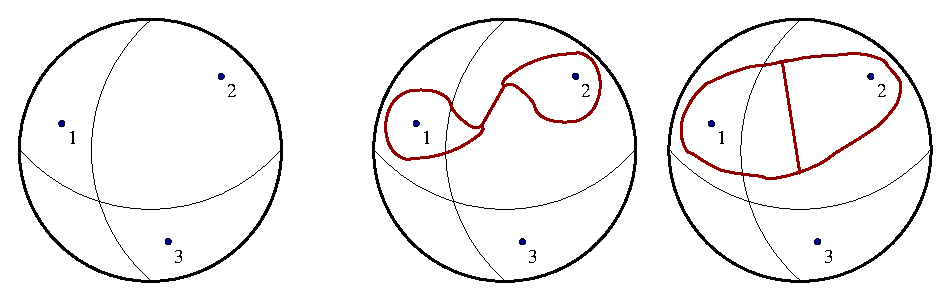
\includegraphics[width=\textwidth]{sfera3}
  \caption{A thrice-punctured sphere and two deformation retracts, not
    isomorphic as graphs.}
  \label{fig:sphere-retracts}
\end{figure}
We can refine this correspondence by introducing more structure on the
graph.
\begin{definition}
  \label{dfn:metric-ribbon-graphs}
  A metrized ribbon graph $(G, \ell)$ is a ribbon graph $G$ equipped with
  a real positive number $\ell_\alpha$ for each edge $\alpha \in \Edges{G}$.
\end{definition}

We can give the topological Riemann surface $S(G)$ a complex
structure by means of a triangulation and an analytic atlas.

In the course of the construction of $S(G)$, two punctured disk have
been glued on the sides of an edge $\alpha \in \Edges{G}$: call them $\alpha^+$
and $\alpha^-$; they are not necessarily distinct.  Let $T_\alpha^+$ and $T_\alpha^-$
be the triangles delimited by $\alpha$ and the radii joining endpoints of
$\alpha$ with the puncture of $\alpha^\pm$. The collection $\{T_\alpha^\pm : \alpha \in
\Edges{G}\}$ is a triangulation of $S(G)$.

Define an atlas of $S(G)$:
\begin{itemize}
\item for any edge $\alpha \in \Edges{G}$, put $V_\alpha := (T_\alpha^+ \cup T_\alpha^-)^\circ$;
\item for any boundary component $\beta \in \Holes{G}$, put $V_\beta := \bigl(
  \bigcup_{\alpha} T_\alpha \bigr)^\circ$ for all $\alpha$ bounding $\beta$;
\item for any vertex $\gamma \in \Vertices{G}$, put $V_\gamma := \bigl( \bigcup_\alpha T_a^\pm
  \bigr)^\circ$ for all $\alpha$ incident to $\gamma$.
\end{itemize}
\begin{figure}[btp]
  %% Figura atlas.fig
  \centering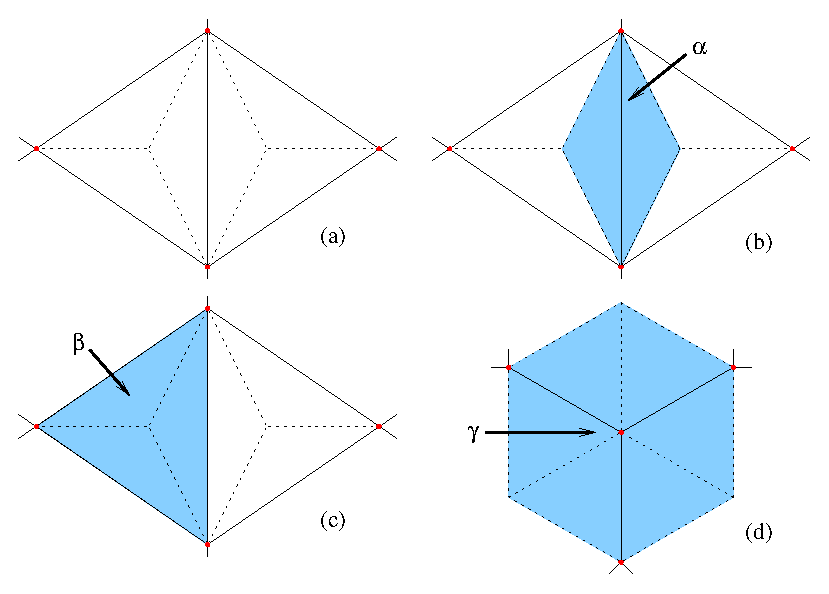
\includegraphics[width=\textwidth]{atlas}
  \caption{The open sets building an atlas of $S(G)$: (a) the
    triangulation built from a graph $G$: graph edges are drawn as
    solid lines, and edges of $T_\alpha^{\pm}$ are drawn as dotted lines; (b)
    the neighborhood $V_\alpha$ of an edge $\alpha$; (c) the neighborhood $V_\beta$
    of a boundary component $\beta$; (d) the neighborhood $V_\gamma$ of a
    vertex $\gamma$.}
  \label{fig:atlas}
\end{figure}

Define charts on the open sets $V_*$ (see Figure~\ref{fig:charts}):
\begin{itemize}
\item for any edge $\alpha$, pick a homeomorphism $f_\alpha: V_\alpha \to \{ z \in \setC
  : 0 < \Re z < \ell_\alpha \}$;
\item for any boundary component $\beta$, bounded by edges $\alpha_1$, $\alpha_2$
  and $\alpha_3$, pick a homeomorphism $f_\beta: V_\beta \to \{ \abs{z} < \rho \}$, where
  $\rho = (\ell_{\alpha_1} + \ell_{\alpha_2} + \ell_{\alpha_3}) / 2\pi$.
\item for any vertex $\gamma$, pick a homeomorphism $f_\gamma: V_\gamma \to \setC$.
\end{itemize}
\begin{figure}[htbp]
  %% Figura charts.fig
  \centering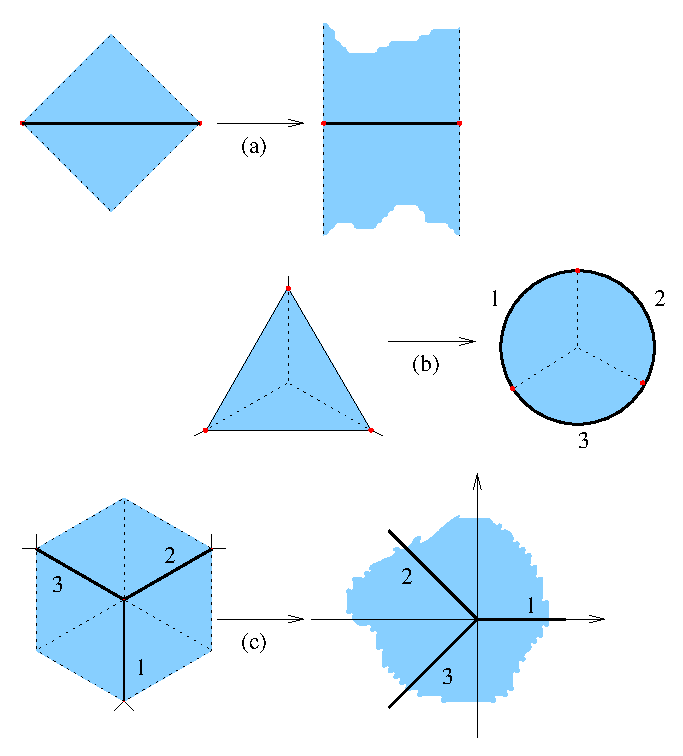
\includegraphics{charts}
  \caption{Local charts on the atlas: (a) any open set $V_\alpha$
    maps to a strip in the complex plane; (b) any open set $V_\beta$
    maps to a disk; (c) any open set $V_\gamma$ maps to the complex
    plane itself.}
  \label{fig:charts}
\end{figure}
These choices are subject to the condition that transition functions
satisfy the following:
\begin{itemize}
\item if $\alpha$ is an edge bounding the hole $\beta$, then $f_\beta \circ
  f_\alpha^{-1} = \exp (2\pi\I z / p_\beta)$ with $p_\beta := \sum_{\alpha \in \beta} \ell_\alpha$
  (\emph{perimeter} of the hole $\beta$);
\item if $\alpha$ is incident to a vertex $\gamma$, then $f_\gamma \circ f_\alpha^{-1} =
  c \cdot z^{2/(v+2)}$, up to a complex constant of modulus $1$, where
  $v$ is the valence of the vertex $\gamma$.
\end{itemize}

In the end, we have come upon a complex analytic structure on $S(G)$,
which depends on the perimeters $p_1, \ldots, p_n$ of boundary components
$\beta_1, \ldots, \beta_n$. By varying these (real positive) parameters, one can
vary the complex structure on $S(G)$; this will allow for a different
construction of the moduli space $\M_{g,n}$.

The perimeters $p_1$, \ldots, $p_n$ depend on the matric data $\ell_\alpha$,
therefore the complex analytic structure on $S(G)$ actually depends on
the metrized graph $(G, \ell)$.  Let $S(G, \ell)$ denote the Riemann
surface $S(G)$ endowed with this complex analytic structure.

\begin{remark}
  Note that the above procedure actually equips any metrized ribbon
  graph $(G, \ell)$ with a structure of embeddded ribbon graph: take the
  obvious $\iota:G \to S(G, \ell)$ as immersion of the graph, and maps $f_\beta$ as
  the homeorphisms between $S \setminus \iota(G)$ and punctured disks.
\end{remark}


\subsection{Construction of $\Tcomb_{g,n}$ and $\Mcomb_{g,n}$}
\label{sec:mgn-comb-construction}

Let $G$ be a metrized ribbon graph of genus $g$ with $n$ numbered
boundary components.  A topological cell $\Delta(G) \subseteq \M_{g,n}$ is spanned
when varying the metric data $(\ell_\alpha)_{\alpha \in \Edges{G}}$; gluing these
cells one recovers the whole $\M_{g,n}$.  A construction of
$\Tcomb_{g,n}$ can be found in \cite{penner:math.GT/0210326}, although
the actual procedure mimicks
\cite{kontsevich;intersection-theory;1992}.

Call a set $X \subseteq \Edges{G}$ negligible whenever it is \emph{not} the
support of a non-trivial homological cycle.  For an abstract ribbon
graph $G$, define:
\begin{equation*}
  \label{eq:rg-cells-moduli}
  \Delta(G) := \{ \ell: \Edges{G} \to \setR_{\geq0} | \text{the zero set of $\ell$ is negligible}\}.
\end{equation*}
It is a contravariant functor from the category of abstract ribbon
graphs to the category of topological spaces: if $G'$ is obtained from
$G$ by contracting the edge $\alpha$, then
\begin{equation}\label{eq:embedding-cells}
  \Delta(G') = \{ \ell \in \Delta(G) | \ell_\alpha = 0 \}.
\end{equation}
By composing with the forgetful functor $[G, \iota, \psi_*] \mapsto G$ from
embedded ribbon graphs to abstract ribbon graphs, we define a
contravariant functor on the category of embedded ribbon graphs:
\begin{equation*}
  \label{eq:rg-cells-teichmueller}
  T\Delta[G, \iota, \psi_*] := \Delta(G).
\end{equation*}

\begin{definition}
  The combinatorial Teichm\"uller space is the direct limit of the
  functor $T\Delta$:\FIXME{%
    In realt\`a, Penner costruisce questo spazio non come limite
    diretto, ma incollando esplicitamente le celle.  C'\`e qualcosa di
    nascosto che non funziona col limite diretto?  Per esempio si fa a
    meno del lemma~\ref{lemma:erg-no-aut}.  }%
  \begin{equation*}
    \Tcomb_{g,n} := \varinjlim T\Delta[G, \iota, \psi_*],
  \end{equation*}
  where $[G, \iota, \psi_*]$ ranges in the category $\ERG{g,n}$ of embedded
  ribbon graphs of genus $g$ with $n$ numbered boundary components.
\end{definition}
$\Tcomb_{g,n}$ is obtained by gluing topological cells $\Delta(G)$ alongside
the boundary: if $[G', \iota', \psi'_*]$ is obtained from $[G, \iota, \psi_*]$ by
contraction of an edge $\alpha$, then $\Delta(G')$ is identified with the face
of $\Delta(G)$ where $\ell_\alpha = 0$ by \csref{eq:embedding-cells}.

Elements of the topological space $\Tcomb_{g,n}$ are (equivalence
classes of) metrized embedded ribbon graphs $[G, \iota, \psi_*, \ell]$, where $\ell
\in T\Delta[G, \iota, \psi_*]$; it is easy to check that any $[G, \iota, \psi_*, \ell] \in
\Tcomb_{g,n}$ has a unique representative such that $\ell_\alpha > 0$ for all
$\alpha \in \Edges{G}$.  Perimeter maps $p_\beta: \Tcomb_{g,n} \to \setR_{>0}$ are
well-defined; write $p_j$ for the perimeter of the $j$-th hole.

\begin{definition}
  The combinatorial moduli space of curves is the direct limit of the
  functor $\Delta$:
  \begin{equation*}
    \Mcomb_{g,n} := \varinjlim \Delta(G),
  \end{equation*}
  where $G$ ranges in the category $\RG{g,n}$ of abstract ribbon
  graphs of genus $g$ with $n$ numbered boundary components.
\end{definition}

The functorial action of $\Gamma_{g,n}$ on $\ERG{g,n}$ induces an action
on $\Tcomb_{g,n}$.
\begin{lemma}
  \label{lemma:penner-kontsevich-bridge}
  $\Mcomb_{g,n}$ is the quotient space (in the orbifold sense) of
  $\Tcomb_{g,n}$ by the action of the mapping class group $\Gamma_{g,n}$.
\end{lemma}
\begin{proof}
  If $G \in \RG{g,n}$ is any abstract ribbon graph, then map $\Delta(G)$ into
  $\Tcomb_{g,n} / \Gamma_{g,n}$ by the following: pick any representative
  embedding ${\tilde G} = [G, \iota, \psi_*] \in \ERG{g,n}$ of $G$ and compose
  the isomorphism $\Delta(G) \cong T\Delta(\tilde G)$ with the quotient
  projection $T\Delta(\tilde G) \to \Tcomb_{g,n}/\Gamma_{g,n}$.  The mapping
  is well-defined: if $[G, \iota, \psi_*]$ and $[G, \iota', \psi'_*]$ are two
  distinct embeddedings of $G$, then ${\tilde \iota}, {\tilde \iota'}: S(G) \to
  S$ are homemorphisms, and, for any $\ell \in \Delta(G)$, $\iota' \circ \iota^{-1}$ is
  differentiable with respect to the analytic structure $S(G, \ell)$.
  Therefore, if $\phi := (\iota')^{-1} \circ \iota$, then $[G, \iota, \psi_*] = \phi \cdot [G, \iota',
  \psi'_*]$.

  By definition of direct limit, a map $\Phi$ is induced $\Mcomb_{g,n} \to
  \Tcomb_{g,n} / \Gamma_{g,n}$.  It is surjective: every point in $\Tcomb /
  \Gamma$ is a projection of a point $[G, \iota, \psi_*] \in \Tcomb$, therefore it
  is in the image of $G \in \Mcomb$.  $\Phi$ is injective: if $G$ and $G'$
  map to the same point in $\Tcomb / \Gamma$, then there is some $\phi \in \Gamma$
  such that $[G, \iota, \psi_*] = \phi \cdot [G', \iota', \psi'_*] = [G', \phi \circ \iota, \psi'_* \circ
  \phi]$; therefore, there is $\phi' \in \Diff^0$ such that $\phi' \circ \iota = \phi \circ \iota'$.
  Thus $f = \iota' \circ \iota^{-1}: G' \to G$ is a isomorphism of ribbon
  graphs.\FIXME{Questa ``dimostrazione'' non mi convince molto.}
\end{proof}

As in the final part of the proof of
\csref{lemma:penner-kontsevich-bridge}, we can see that the image
$M(G) \subseteq \Mcomb$ of a cell $\Delta(G)$ is the quotient of $\Delta(G)$ by $\Aut
G$.  The orbicells $M(G)$ are glued alongside the boundary, according
to the same procedure as in $\Tcomb$: if $G'$ is a contraction of $G$,
then $M(G')$ is a face of $M(G)$). Therefore, $\Mcomb_{g,n}$ is a
orbifold.

The cell $M(G)$ has real dimension $\card{\Edges{G}}$; therefore,
cells of maximal dimension are given by graphs with all vertices of
valence $3$. The union of these cells is a dense subset of
$\Mcomb_{g,n}$ with non-void interior.

\subsubsection{Kontsevich' compactification of $\Mcomb_{g,n}$}
\label{sec:comp-mcomb}
The construction of $\Mcomb_{g,n}$ can be done with slightly changed
rules: if we define a set $X \subseteq \Edges{G}$ to be negligible iff it does
not contain \emph{all} edges bounding a hole, then we can define a
contrafunctor $\overline{M}(G)$ and a topological space:
\begin{equation*}
  \label{eq:kontsevich-4}
  \Mbarcomb_{g,n} := \varinjlim \overline{M}(G).
\end{equation*}
$\Mbarcomb_{g,n}$ turns out to be a compactification of the orbifold
$\Mcomb_{g,n}$. 


\subsection{From surfaces to graphs: the Jenkins-Strebel Theorem}
\label{sec:strebel}
A theorem proved independently by J.~A. Jenkins \cite{jenkins;annals}
and K.~Strebel \cite{strebel;quadratic-differentials;1983} provides
the key tool for the inverse route: the construction of ribbon graphs
from smooth complex curves.

\begin{definition}
  A quadratic differential $q$ on a Riemann surface $S$ is a
  (meromorphic) section of $(T^*S)\tp2$.
\end{definition}
The set of vectors in $T_zS$ on which $q$ takes real non-negative
values forms a real line in $T_zS$: therefore, they make up a
foliation $F = F_qS$ on $S \setminus \{\text{poles of $q$}\}$. The non-compact
leaves of $F$ together with zeroes of $q$ form the ``critical locus''
of $q$.  Call $F$ the ``horizontal'' foliation associated with $q$.

The set of vectors in $T_zS$ on which $q$ takes a purely imaginary
value form a perpendicular foliation $F^\perp$, whose leaves connect
either two distinct poles $x_i$ and $x_j$, or a pole $x_i$ and a zero
$v_j$.  Call $F^\perp$ the ``vertical'' foliation associated with $q$.

Every quadratic differential $q$ induces a metric (away from the
critical locus) by $\ud s^2 = \abs{q(z)} \cdot \abs{\ud z}$.

\begin{theorem}[Jenkins, Strebel; {\cite[Theorem 23.2 and
    23.5]{strebel;quadratic-differentials;1983}}] 
  \label{thm:JS}
  For any complex analytic curve $S$ with $n$ marked points $x_1, \ldots,
  x_n$, and any assignment of real positive numbers $p_1, \ldots, p_n$,
  there exists one and only one quadratic differential $q$ such that:
  \begin{itemize}
  \item the only poles of $q$ occur at the marked points $x_1, \ldots, x_n$
    with second residue $p_1, ..., p_n$, that is, in a local
    coordinate $z_i$ near $x_i$ we have:
    \begin{equation*}
      q = -p_i^2 (\d z_i^2 / z_i^2) + \text{higher order terms};
    \end{equation*}
  \item the non-critical real trajectories of $F_q$ are simple closed
    circles around $x_i$.
  \end{itemize}
  Furthermore, $q$ has the following properties:
  \begin{itemize}
  \item every nonsingular closed leaf circling around $x_i$ has length
    $p_i$ in the flat metric induced by $q$.
  \item the critical locus of $q$ is a graph $G$ embedded in $S$;
  \item the complement $S \setminus G$ of the critical locus is a collection
    of disks $\{D_i | i=1,\ldots,n\}$, each one centered at a pole $x_i$, and
    the projective class of the collection of radii of disks $\{D_i\}$
    equals the projective class $[p_1, \ldots, p_n]$.
  \end{itemize}
\end{theorem}
The critical graph $G$ inherits a structure of embedded ribbon graph
with metric from the ambient surface $S$: the length of an edge $\alpha$ is
the one measured in the metric induced by the quadratic differential.
Furthermore, Jenkins-Strebel's theory states that $G$ has a vertex of
valence $k+2$ where $q$ has a zero of order $k$, therefore, vertices
of $G$ have valence $\geq3$. 

Since the markings $x_1, \ldots, x_n$ are \emph{ordered}, $G$ has an
additional structure of \emph{numbered} graph, that is, it is endowed
with a bijection $h: \Holes{G} \to \{1, \ldots, n\}$.


\subsection{Relation with $\M_{g,n}$ and $\T_{g,n}$}
\label{sec:nocomb}

\begin{theorem}[Harer, Mumford, Thurston;
  \cite{harer;cohomological-dimension,
    looijenga;cellular-decomposition, penner:math.GT/0210326}] 
  The Jenkins-Strebel construction defines morphisms
  \begin{equation*}
    \T_{g,n} \times \setR_{>0}^n \to \Tcomb_{g,n}, 
    \qquad
    \M_{g,n} \times \setR_{>0}^n \to \Mcomb_{g,n}, 
    \qquad 
    \Mbar_{g,n} \times \setR_{>0}^n \to \Mbarcomb_{g,n}.
  \end{equation*}
  The first of these is a homeomorphism and the second is an orbifold
  equivalence. 

  The inverse map
  \begin{equation*}
    \Tcomb_{g,n} \to \T_{g,n} \times \setR_{>0}^n \to \setR_{>0}^n,
    \qquad
    \Mcomb_{g,n} \to \M_{g,n} \times \setR_{>0}^n \to \setR_{>0}^n
  \end{equation*}
  is the perimeter map $\pi := (p_1, \ldots, p_n)$.  
\end{theorem}

For any given $p^\circ = (p_1^\circ, \ldots, p_n^\circ) \in \setR_{>0}^n$, the fiber
$\pi^{-1}(p^\circ)$ is isomorphic to $\M_{g,n}$ (resp.\ $\T_{g,n}$), thus,
$\pi$ induces a triangulation of $\M_{g,n}$ (resp.\ $\T_{g,n}$).



\section{Harer's equivariant spine for Teichm\"uller space}
\label{sec:spine}

Harer \cite{harer;cohomological-dimension}, introduced a simplicial
spine for the Teichm\"uller space $\T_{g,n}$.  

If $X$ is any semi-simplicial complex, denote by $|X|$ its geometric
realization.  Denote by $X'$ the first barycentric subdivision of $X$,
that is, $X'$ has a $k$-simplex $(\sigma_0 > \sigma_1 > \cdots > \sigma_k)$ for any chain
of $k+1$ simplices in $X$ such that $\sigma_{i+1}$ is a face of $\sigma_i$.


\subsection{Arc-systems}
\label{sec:arc-systems}

Let $T_{g,n}$ be a topological compact oriented Riemann surface of
fixed genus $g$ with $n$ marked points $x_1, \ldots, x_n$.  Regard points
in the moduli space $\M_{g,n}$ as equivalence classes $(S,x,\varphi)$ of a
complex analytic curve $S$ with a marking $x:\{1,\ldots,n\}\to S$ and a
homeomorphism $\varphi:S\to T_{g,n}$ with the reference surface (see
\csref{sec:alternate-Mgn}).

If $u$ is any arc in $S$, denote by $[u]$ its isotopy class rel~$\{x_1,
\ldots, x_n\}$.
\begin{definition}
  An arc-system $[u_1, \ldots, u_k]$ of rank $k$ is an isotopy class
  rel~$\{x_1, \ldots, x_n\}$ of $k$ properly imbedded arcs $u_i : [0,1] \to S$
  such that:
  \begin{itemize}
  \item every $u_i$ has its endpoints in the set $\{x_1, \ldots, x_n\}$;
  \item if $i \neq j$, then $u_i$ meet $u_j$ only at endpoints, if at all;
  \item no $u_i$ is null-homotopic rel~$\{x_1, \ldots, x_n\}$;
  \item no $u_i$ is homotopic rel~$\{x_1, \ldots, x_n\}$ to $u_j$, for $i \neq
    j$;
  \end{itemize}
  An arc-system $[u_1, \ldots, u_k]$ is said to \emph{fill up} the curve
  $S$ iff all connected components of $S - \bigcup\{u_i\} - \{x_1,\ldots x_n\}$ are
  either disks or once-punctured disks.
\end{definition}
Note that a connected component of the complement of a filling
arc-system can only be punctured at a marked point $x_i$.

Arc-systems may be organized into a semi-simplicial complex.
\begin{definition}
  $U$ is the semi-simplicial complex having a simplex $\langle u_1, \ldots, u_k\rangle$
  for every rank $k$ arc-system $[u_1, \ldots u_k]$, with the proviso that
  $\langle u'_1, \ldots, u'_l\rangle$ is a face of $\langle u_1, \ldots, u_k\rangle$ iff $\{ [u'_1], \ldots,
  [u'_l] \} \subset \{ [u_1], \ldots, [u_k] \}$.
  
  $U_0$ is the subcomplex of all those simplices $\langle u_1, \ldots, u_k\rangle$
  that do not fill up the surface $S$.
\end{definition}
By definition of $U_0$, any simplex in $U$ whose vertices are a subset
of the vertices of $\sigma_\bullet \in U_0$ is itself a simplex in $U_0$.

Let $U'$, $U_0'$ be the first barycentric subdivisions of $U$
and $U_0$, respectively.

There is a natural action of $\tau \in \Gamma_{g,n}$ on $U$ given by $\tau \cdot [u_1, \ldots
u_k] := [\tau \circ u_1, \ldots, \tau \circ u_k]$; it preserves $U_0$, so it restricts to
an action on $U \setminus U_0$.

Let $\Delta^{n-1}$ be the $(n-1)$-dimensional geometric simplex.
\begin{theorem}[Harer, {\cite[Theorem
    1.3]{harer;cohomological-dimension}}]
  \label{thm:H}
  There exists a $\Gamma_{g,n}$-equivariant homeomorphism $\Phi: \T_{g,n} \times
  \Delta^{n-1} \to |U \setminus U_0|$.
\end{theorem}
This is infact another application of \csref{thm:JS1}.  We only sketch
part of proof here in order to highlight the features needed in the
sequel. 

Given a marked complex analytic curve $S$, and barycentric coordinates
$b_0 + \cdots + b_n = 1$, by Jenkins-Strebel's \csref{thm:JS1}, there is a
quadratic differential $q$ that has poles at the marked points $\{ x_1,
\ldots, x_n \}$ such that its second residue at $x_i$ is $b_i$.

Form the horizontal and vertical foliations $F$, $F^\perp$ induced by $q$,
as in \ref{sec:strebel}.  Leaves of $F^\perp$ either connect a marked
point $x_i$ (a pole of $q$) to another pole or to a zero point of $q$.
Let $F^\perp_0$ be the collection of leaves of $F^\perp$ that join poles of
$q$; it breaks up into parallel families, where two leaves are
parallel iff they are connected by a homotopy in $S$ fixing the zeroes
and the poles of $q$.  Select one leaf $u_j$ from each family, and
form an arc-system $u = [u_1, \ldots, u_k]$.

Let $G$ be the critical graph of $q$.  Each edge $\alpha \in \Edges{G}$ meets
only \emph{one} arc $u_i$, and they intersect transversally and at one
point only.  Therefore we can associate with every arc $u_i$ the
$q$-length $\ell_i$ of the unique edge $\alpha$ intersecting $u_i$.  

Let $\Phi(S, b_*)$ be the point in the geometric simplex $|\langle u_1, \ldots u_k\rangle|$
corresponding to the projective class $[\ell_1:\cdots:\ell_k]$.  This defines a
map $\Phi$ from $\T_{g,n} \times \Delta^n$ to $|U \setminus U_0|$, which is
proven to be a homeomorphism \cite{harer;cohomological-dimension,
  harer;cohomological-dimension,looijenga;cellular-decomposition}.

\begin{remark}
  \label{rem:approaching-face}
  When the length $\ell_j$ approaches $0$, the point $\Phi(S, b_*)$
  approaches a point on a face of the simplex $|\langle u_1, \ldots, u_k\rangle|$; this
  face is identified with the simplex $|\langle u_1, \ldots, \hat{u_j}, \ldots, u_k\rangle|$.
\end{remark}


\subsection{The equivariant spine for $\T_{g,n}$}
\label{sec:spine}

\begin{definition}
  Let $Y'$ be the collection of simplices in $U'$ having no face in
  $U_0'$; equivalently, $\sigma_\bullet \in Y'$ iff every vertex of $\sigma_\bullet$
  lies in $U' \setminus U_0'$.
\end{definition}
$Y'$ is a full subcomplex of $U'$; vice versa, if $(\sigma_0 > \sigma_1 > \cdots >
\sigma_k) \in Y'$, then \emph{no} $\sigma_i$ belongs to $U_0'$.  

It can be proved that $Y'$ is 

The action of $\Gamma_{g,n}$ on $U'$ preserves $Y'$.
\begin{theorem}[Harer, {\cite[theorem
    2.1]{harer;cohomological-dimension}}]
  \label{thm:spine}
  The semi-simplicial complex $U'$ has an equivariant deformation
  retraction on $Y'$.  This retraction provides a
  $\Gamma_{g,n}$-equivariant homotopy equivalence between $U' \setminus U_0'$ and
  $Y'$.
\end{theorem}

The complex $Y'$ is isomorphic to the first barycentric subdivision of
a $4g - 5 + 2n$ dimensional complex $Y$, the dual complex to $U'$,
constructed as follows:
\begin{itemize}
\item $Y$ has a 0-simplex for every maximal arc-system that fills up the
  reference surface $T$; each such arc-system has $N = 6g - 7 + 3n$ arcs.
\item $Y$ has a 1-simplex for every arc-system formed by $N-1$ arcs:
  each such arc-system has two completions to a maximal arc-system.
\item By recursively iterating this construction, we can construct the
  higher-dimensional simplices in $Y$.\FIXME{Non \`e cos\`\i{} ovvio:
    bisogna mostrare che i completamenti di un arc-system dato ad uno
    massimale si organizzano in un simplesso.  Harer usa un teorema di
    struttura per il complesso degli arc-system. Ma forse l'intera
    descrizione di $Y$ pu\`o essere omessa qui, perch\'e ci interessa solo
    il complesso dei grafi a nastro.}
\end{itemize}
Notice that, at a minimum, $2g - 2 +n$ curves are required to fill up
$T$, so $Y$ is $4g - 5 + 2n$ dimensional.



\section{The ribbon graph complex}
\label{sec:ribbon-graph-complex}

Finally, we can translate Harer's spine in terms of ribbon graphs and
use it to construct a complex that computes the homology of
$\M_{g,n}$.  The route to it is a bit convoluted, as the direct
approach to constructing a ribbon graph complex by defining face
operators through admissible contractions does not yield a simplicial
complex: after a few contractions, loops appear, which cannot be
contracted any more.  This mirrors the structure of $U \setminus U_o$, as will
be shown in \ref{sec:contractions-and-topology}.

\begin{definition}
  \label{dfn:rg-complex}
  Let $\R$ be the semi-simplicial complex whose vertices are
  \emph{abstract} ribbon graphs, and whose face operators are given by
  admissible contractions.
\end{definition}
In other words, given ribbon graphs $G$ and $G'$, we identify $G'$
with a face of $G$ iff there exists a non-loop edge $\alpha \in \Edges{G}$
such that $G'$ is the contraction of $G$ by $\alpha$.

Similarly, we construct the complex of embedded ribbon graphs.
\begin{definition}
  \label{dfn:erg-complex}
  Let $\tilde\R$ be the semi-simplicial complex whose vertices are
  \emph{embedded} ribbon graphs, and whose face operators are given by
  admissible contractions.
\end{definition}

The mapping class group $\Gamma_{g,n}$ acts on $\tilde\R$ by changing the
embedding; we have $\R_{g,n} \simeq \tilde\R_{g,n} / \Gamma_{g,n}$.


\subsection{From arc-systems to ribbon graphs}
\label{sec:arcs-to-rg}

Let $u = [u_1, \ldots, u_k]$ be an arc-system on $T_{g,n}$ uniquely
labeling a simplex $\Delta(u)$ in $U \setminus U_0$.  Any choice of barycentric
coordinates $b_0 + \cdots + b_k = 1$ in $\Delta(u)$ identifies a point in $|U \setminus
U_0|$.  By the proof of Harer's \csref{thm:H} this corresponds to a
complex structure on $T_{g,n}$ (a point in $\T_{g,n} \times \Delta^n$)
determined by a quadratic differential $q = q(u, b_*)$, such that each
arc $u_i$ is a regular curve in the vertical foliation $F^\perp$
associated to $q$.

Let $G$ be the critical graph of $q$.  By the statement and the
remarks following \csref{thm:JS1}, $G$ has the structure of a
\emph{embedded} ribbon graph.

Let $\alpha_k$ be the only edge of $G$ meeting the arc $u_k \in u$; we can
put a metric on $G$ by letting the length of $\alpha_k$ be $b_k$, the
barycentric coordinate on the side of $u_k$.  Therefore $G$ has the
structure of a \emph{metrized} embedded ribbon graph.

By the 1-1 correspondence of arcs in $u$ and edges of $G$, any order
of the vertices of $\Delta(u)$ translates to an order of the edges of $G$.

We can sum up the above construction in the following statement.
\begin{lemma}
  \label{lemma:arcs-to-rg}
  There's a 1-1 correspondence between arc-systems $u \in U \setminus U_0$ and
  embedded ribbon graphs in $\tilde G \in \ERG[g,n]$; $\tilde G$ is the
  dual graph to $u$ in the ambient surface $T_{g,n}$.

  To any point in $|U \setminus U_0|$, there corresponds a \emph{metrized}
  embedded ribbon graph, the barycentric coordinates in simplexes of
  $|U \setminus U_0|$ directly translating to edge-lengths of $\tilde G$.

  Finally, if an order of the vertices of the simplex $\Delta(u)$ is given,
  then an order of the edges of $\tilde G$ is induced.
\end{lemma}


\subsection{Contraction of edges and the cell complex structure}
\label{sec:contractions-and-topology}

In \csref{sec:arcs-to-rg}, a PL isomorphism was actually constructed
between the geometric simplex $|\langle u_*\rangle|$ and $|\tilde G|$, the
geometric simplex spanned by varying lengths of edges in
$\Edges{\tilde G}$.  By \csref{lemma:approaching-face}, the face
operators on the two set of simplices are compatible with this PL
isomorphism, so we can glue isomorphisms $|\langle u_*\rangle| \to |G|$ to form a PL
isomorphism $|U \setminus U_0| \to \Tcomb_{g,n}$.

Recall that the cells that make up $\Tcomb_{g,n}$ are indexed by
embedded ribbon graphs, and let $\tilde G \in \ERG[g,n]$ be an embedded
ribbon graph. If no edge of $\tilde G$ is a loop, then any contraction
of an edge in $\tilde G$ produces an embedded ribbon graph in
$\ERG[g,n]$, which again corresponds to a simplex in $U \setminus U_0$.
Therefore, embedded ribbon graphs with no loops identify cells
entirely contained in $U \setminus U_0$. 

Now let $\tilde G$ be an embedded ribbon graph having a loop $\lambda \in
\Edges{G}$, and let $u = \langle u_1, \ldots, u_k\rangle$ be the arc-system simplex
corresponding to $\tilde G$ according to \csref{lemma:arcs-to-rg}.
Contraction of $\lambda$ in $\tilde G$ is not admissible, as it would change
the genus and/or the puncture number of $\tilde G$.  Correspondingly,
if $u'$ be the face of $u$ obtained by omitting the unique arc
that intersects $\lambda$, then $u'$ does not fill up the ambient surface.

Vice versa, suppose that $u' \in U_0$ is such that adding a single arc
$u_0$ to $u'$ determines a simplex belonging to $U \setminus U_0$.  Let
$\tilde G$ be the embedded ribbon graph, dual to $\langle u_0, u'\rangle$.  It's
simple to see then:
\begin{enumerate}
\item The arc $u_0$ is entirely contained in a connected component $W$
  of $T \setminus |u'|$, and this $W$ is either a punctured disk or a disk
  with a slit in the middle.  Indeed, let $W' := W \setminus |u_0|$; since
  $\langle u_0, u'\rangle$ belongs to $U \setminus U_0$, then $W'$ is a topological disk.
  The border of $W'$ is union of the arcs $u_i$, where each arc occurs
  at most two times, and, for those that occur two times, the two
  copies have equal length in the metric of $T$.  The arc $u_0$ occurs
  two times on the border of $W'$, and we get $W$ by isometrically
  gluing $W'$ along the two copies of $u_0$. 
\item The arc $u_0$ connects the puncture or slit in $W$ with the
  border of $W$.
\item The edge $\lambda$ of $\tilde G$ corresponding to $u_0$ is a loop.
\end{enumerate}

The following sums up the content of this section.
\begin{lemma}
  \label{lemma:erg-loop}
  Embedded ribbon graphs with a loop correspond to arc-system simplices
  in $U$ with a face on $U_0$; every loop in a ribbon graph $\tilde G$
  corresponds to a face on $U_0$ in the dual arc-system.
\end{lemma}



%%% Local Variables: 
%%% mode: latex
%%% TeX-master: "index"
%%% x-symbol-8bits: nil
%%% End: 
